
Let 
    \begin{align}
    &\angle B= 105\degree=\theta \label{quad/42/eq1}
    \\
    &\angle C= 80\degree=\alpha \label{quad/42/eq2}
    \\
    &\norm{\vec{A}-\vec{B}} =4=p \label{quad/42/eq3}
    \\
    &\norm{\vec{C}-\vec{B}} =5=q \label{quad/42/eq4}
    \\
     &\norm{\vec{D}-\vec{C}} =6.5=r \label{quad/42/eq5}
    \end{align}
and 
\begin{align}
    &\vec{B}=\myvec{0\\0}, \vec{C}=\myvec{5\\0}
\end{align}

\begin{lemma}
\label{quad/42/lemma}
\begin{align}
  & \vec{A} = p \vec{b}  \quad \brak{\because \vec{B}=\myvec{0\\0}} \label{quad/42/eq a}
\\
  & \vec{D} =\vec{C} + r \vec{c} \label{quad/42/eq b}
\end{align}
where 
\begin{align}
 \vec{b} = \myvec{\cos B \\ \sin B } ,\vec{c} = \myvec{\cos C\\ \sin C }
\end{align}
\end{lemma}
Thus, 
\begin{align}
 \vec{A} &=4\myvec{\cos 105 \\\sin 105 }
\\
&=\myvec{-1.03\\3.86}
\end{align}
and 
\begin{align}
\vec{D} &=\myvec{5\\0} + 6.5\myvec{\cos 80 \\\sin 80 }
\\
&=\myvec{6.12\\6.39}
\end{align}
which are then used to plot Fig. \ref{quad/42/fig:Quadrilateral ABCD}	
\begin{figure}[!ht]
\centering
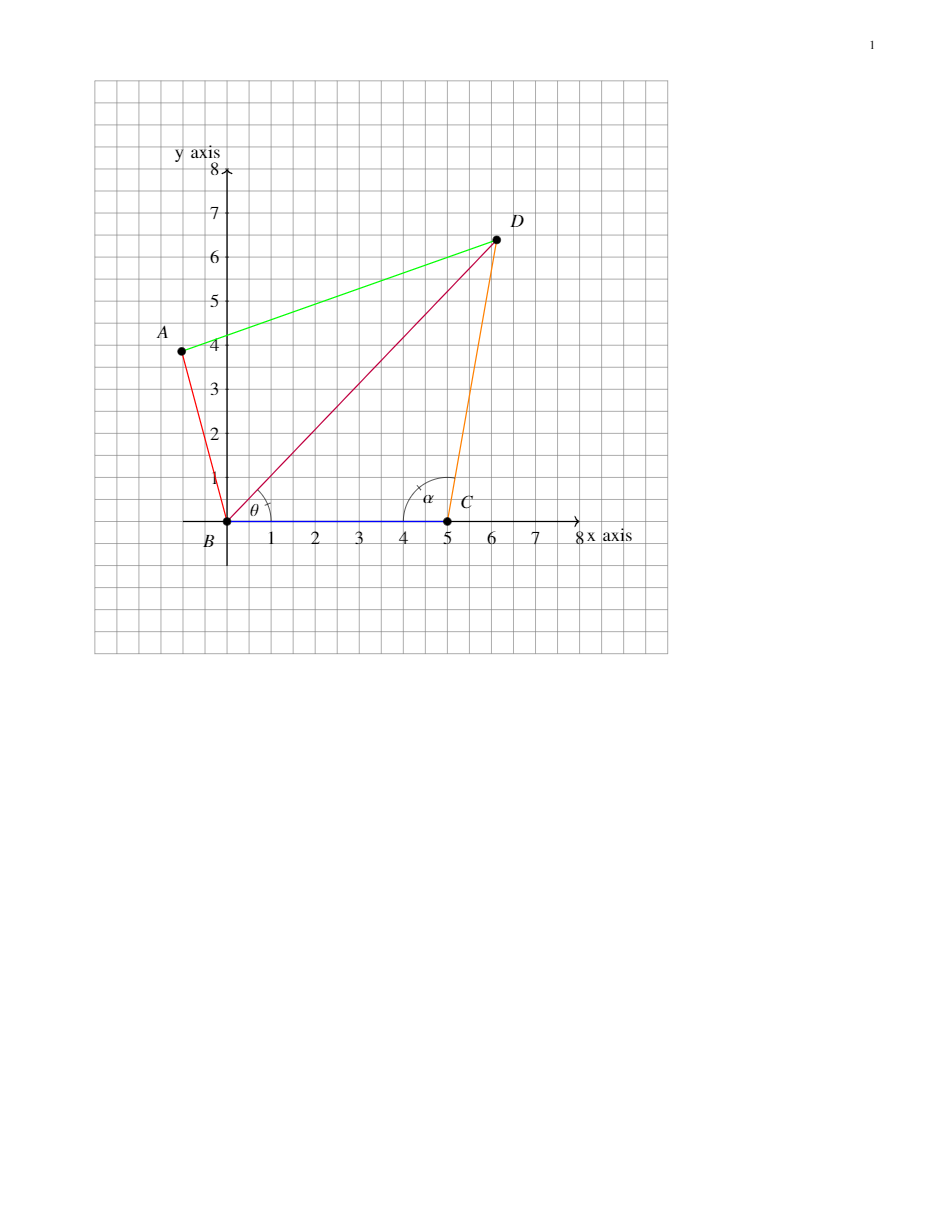
\includegraphics[ width=\columnwidth]{solutions/quad/42/FIGURE.png}
\caption{Quadrilateral ABCD}
\label{quad/42/fig:Quadrilateral ABCD}	
\end{figure}
